\section{Benchmarks}
Im Kapitel \textquote{Benchmarks} geht es darum, ein Gef�hl f�r die Zeitaufw�nde zu bekommen. Dar�ber hinaus werden bestimmte Szenarien mit unterschiedlichen Parametern durchgespielt, um eine Abw�gung von Sicherheit und Performance durchf�hren zu k�nnen.\par

Alle Messungen werden auf Basis des bestehenden Quellcodes mit Hilfe der \textquote{time}-Bibliothek in Python durchgef�hrt. Um Schwankungen auszugleichen, besteht jedes Messergebnis aus dem Durchschnitt von zehn durchgef�hrten Messungen. Gemessen werden dabei immer folgende vier Zeiten:

\begin{enumerate}
	\item Faktoren hashen (kurz \textit{HAS})
	\item Hashwerte in Zahlen umwandeln (kurz \textit{NUM})
	\item Primzahl erzeugen (kurz \textit{PRI})
	\item Shares erzeugen (kurz \textit{GEN})
\end{enumerate}

Wie \autoref{code:measure_time} zeigt, werden die Ergebnisse dabei in Nanosekunden ausgegeben.

\begin{lstlisting}[caption={Vorgehen bei einer Zeitmessung},label=code:measure_time,numbers=left]
start_time = time.time_ns()
# ...
end_time = time.time_ns()
print(end_time - start_time)
\end{lstlisting}

Die Parameter f�r Passwort, Fingerabdruck und Wiederherstellungsschl�ssel sind bei jedem Durchgang identisch und entsprechen folgenden Werten:
    
\begin{itemize}
	\item \textit{Passwort:} 40iOMv9X!*R+
	\item \textit{Fingerabdruck:} 11011000010000011110010010100110
	\item \textit{Wiederherstellungsschl�ssel:} e0b2909559fc9b13e3efefbe868960f6
\end{itemize}

\subsection{Messung des Ist-Stands}

Um eine Vergleichsbasis zu schaffen, werden zuerst Zeitmessungen ohne Anpassungen am Code durchgef�hrt. Mit Blick auf \autoref{chart:measure_ist} l�sst sich ein deutlicher Unterschied zwischen den gemessenen Werten erkennen. Besonders sticht dabei die Berechnung der Primzahl heraus, welche durchschnittlich �ber 1,5 Sekunden lang dauert. W�hrend der Durchf�hrung ist aufgefallen, dass die Primzahlberechnung trotz identischer Eingabeparameter stark schwankt und dabei Zeitaufw�nde zwischen 0,55 und 3,7 Sekunden ben�tigt.\par
Alle anderen Zeiten bewegen sich im Bereich von Bruchteilen einer Sekunde mit Werten von 0.000067 Sekunden (GEN) bis 0.00012 Sekunden (HAS). Die Erzeugung der Shares verl�uft dabei am schnellsten.

\begin{figure}[!h]
\centering
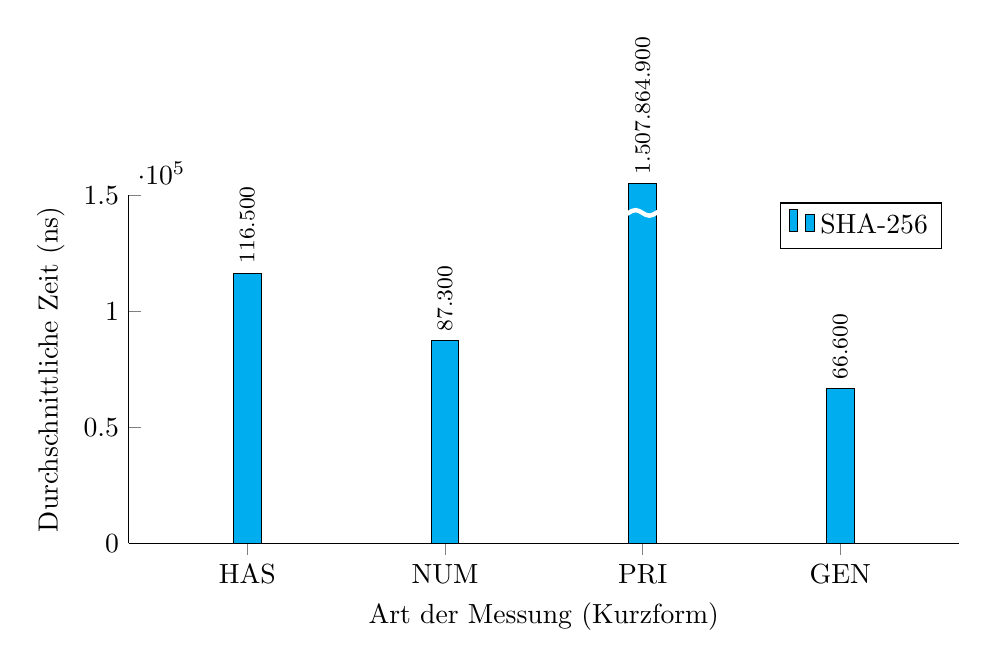
\begin{tikzpicture}
\begin{axis}[
    every axis plot post/.style={/pgf/number format/fixed, /pgf/number format/1000 sep={.}},
    ybar=5pt,
    bar width=10pt,
    width=\linewidth,
    height=6cm,
    ymin=0,
    axis on top,
    ymax=150000,
    xtick=data,
    xlabel={Art der Messung (Kurzform)},
    ylabel={Durchschnittliche Zeit (ns)},
    enlarge x limits=0.2,
    symbolic x coords={HAS,NUM,PRI,GEN},
    restrict y to domain*=0:155000, % Cut values off
    visualization depends on=rawy\as\rawy, % Save the unclipped values
    after end axis/.code={ % Draw line indicating break
        \draw [ultra thick, white, decoration={snake, amplitude=1pt}, decorate] (rel axis cs:0.5,0.95) -- (rel axis cs:1,0.95);
    },
    nodes near coords={
        \pgfmathprintnumber{\rawy} % Print unclipped values
    },
    every node near coord/.append style={font=\footnotesize},
    nodes near coords align={vertical},
    nodes near coords style={rotate=90, anchor=west},
    axis lines*=left,
    clip=false
    ]
\addplot[fill=cyan] coordinates {(HAS, 116500) (NUM, 87300) (PRI, 1507864900) (GEN, 66600)};
\legend{SHA-256}
\end{axis}
\end{tikzpicture}
\caption{Ergebnis: Messung des Ist-Stands}
\label{chart:measure_ist}
\end{figure}

\subsection{Messung mit 512 Bit}

Anstatt SHA-256 wird nun SHA-512 als Hashfunktion f�r den gesamten Prozess verwendet. Die Eingabeparameter bleiben unver�ndert. Eine Umstellung von 256 Bit auf 512 Bit bewirkt sowohl eine Verdopplung der Bitl�nge aller Hashwerte als auch eine Verdopplung der Bitl�nge des Geheimnisses. Auf diesem Geheimnis erfolgt die Berechnung der Primzahl, welche sich unter Verwendung von SHA-256 in der Regel in einer Gr��enordnung von 1536 Bit ($3 \text{ \textit{(Faktoren)} } * 256 \text{ \textit{(Bit)} } * 2$) bewegt und nun durch SHA-512 auf $3072$ Bit anw�chst.\par

Diese Ver�nderungen spiegeln sich in den Zeitmessungen wider, welche in \autoref{chart:measure_512} mit den vorherigen Ergebnissen gegen�bergestellt werden. Allgemein ist wie erwartet eine steigende Tendenz aller Zeiten zu erkennen. Eine auffallend schlechtere Performance ist bei der Berechnung der Shares und der Erzeugung der Primzahl zu verzeichnen. Ersteres ben�tigt mit SHA-512 mehr als doppelt so lange, bei der Primzahl verzehnfacht sich sogar die Zeit, die durchschnittlich w�hrend dieses Prozesses verstreicht. In Zahlen ausgedr�ckt bedeutet dieser Anstieg eine l�ngere Wartezeit von 12,43 Sekunden im Vergleich zu vorher.\par

Es l�sst sich also festhalten, dass die Wahl der Hashfunktion einen essenziellen Einfluss auf die Performance des vorgestellten Verfahrens hat. Bei h�heren Anforderungen an die langfristige Sicherheit des Systems ist dementsprechend in Erw�gung zu ziehen, die neuere SHA-3 (Keccak) Hashfunktion einzusetzen, anstatt die Bits auf 512 zu erh�hen. In weitergehenden Tests konnten allerdings keine erw�hnenswerten Performanceverbesserungen durch die Verwendnung von SHA-3-512 anstelle von SHA-2-512 festgestellt werden.

\begin{figure}[!h]
\centering
\begin{tikzpicture}
\begin{axis}[
    every axis plot post/.style={/pgf/number format/fixed, /pgf/number format/1000 sep={.}},
    ybar=5pt,
    bar width=10pt,
    width=\linewidth,
    height=6cm,
    ymin=0,
    axis on top,
    ymax=250000,
    xtick=data,
    xlabel={Art der Messung (Kurzform)},
    ylabel={Durchschnittliche Zeit (ns)},
    enlarge x limits=0.2,
    symbolic x coords={HAS,NUM,PRI,GEN},
    restrict y to domain*=0:255000, % Cut values off
    visualization depends on=rawy\as\rawy, % Save the unclipped values
    after end axis/.code={ % Draw line indicating break
        \draw [ultra thick, white, decoration={snake, amplitude=1pt}, decorate] (rel axis cs:0.5,0.95) -- (rel axis cs:1,0.95);
    },
    nodes near coords={
        \pgfmathprintnumber{\rawy} % Print unclipped values
    },
    every node near coord/.append style={font=\footnotesize},
    nodes near coords align={vertical},
    nodes near coords style={rotate=90, anchor=west},
    axis lines*=left,
    clip=false,
    legend style={at={(axis description cs:0.45,1.25)}, anchor=north east}
    ]
\addplot[fill=cyan] coordinates {(HAS, 116500) (NUM, 87300) (PRI, 1507864900) (GEN, 66600)};
\addplot[fill=othorange] coordinates {(HAS, 154000) (NUM, 96600) (PRI, 13942158400) (GEN, 172100)};
\addplot[fill=purple] coordinates {(HAS, 119100) (NUM, 87800) (PRI, 16579200800) (GEN, 173000)};
\legend{SHA-256, SHA-512, SHA3-512}
\end{axis}
\end{tikzpicture}
\caption{Ergebnis: Messung mit 512 Bit}
\label{chart:measure_512}
\end{figure}

% Ausprobieren:
%	- SHA-512 statt SHA-256
%	- Gro�e Primzahl (3000 Bits)